\chapter{Unidades de Información digital}

A la hora de almacenar información digital es importante conocer el tamaño del objeto que queremos almacenar y el espacio libre del lugar en el que lo queremos guardar.

En decimal estamos acostumbrados a contar usando el \href{https://es.wikipedia.org/wiki/Sistema_Internacional_de_Unidades}{Sistema Internacional de Unidades}, y dependiendo de la magnitud que queramos medir, haremos uso de unos prefijos establecidos. Por ejemplo, para medir la distancia usamos el \textbf{metro}, y por tanto nos quedaría:

\begin{itemize}
    \item \textbf{Sin prefijo} : metro, una unidad.
    \item \textbf{deca-}metro: $10^1$ metros
    \item \textbf{hecto-}metro: $10^2$ metros
    \item \textbf{kilo-}metro: $10^3$ metros
    \item \textbf{mega-}metro: $10^6$ metros
    \item \textbf{giga-}metro: $10^9$ metros
    \item ...
\end{itemize}

En decimal hacemos uso de la \textbf{base 10}, y por tanto  con cada prefijo lo que estamos haciendo es modificar el exponente que indica la cantidad. Para unidades pequeñas el exponente varía de uno en uno, pero a partir de cierta cantidad (\textbf{kilo-}), la cantidad cambia multiplicando por 1000 ($10^3$).


\section{Sistema binario}

En informática la información se guarda en formato binario, y la unidad más pequeña es el \textbf{bit}, que es un acrónimo de \textit{\textbf{bi}nary digi\textbf{t}}. Cada bit es una única unidad que sólo permite dos estados: \textbf{0} o \textbf{1}. A la hora de representarlo se hace uso de la letra \textbf{b} minúscula, por lo tanto, \textbf{10b} son 10bits.


\subsection{Múltiplos}

Al igual que en decimal, a medida que aumentamos la cantidad, se hace uso de prefijos para facilitar el conocer de qué cantidad estamos hablando.

A continuación se expone una tabla de las medidas más utilizadas:

\begin{yukitblr}{X X X}
    Nombre & Símbolo & Cantidad \\
    \textbf{Bit} & \textbf{b} & $2^0=1$ \\
    Nibble & & 4b \\
    \textbf{Byte} & \textbf{B} & 8b \\
    \textbf{Kibi}byte & \textbf{KiB} & $2^{10}=1024 B$ \\
    \textbf{Mebi}byte & \textbf{MiB} & $2^{20}=1024 KiB$ \\
    \textbf{Gibi}byte & \textbf{GiB} & $2^{30}=1024 MiB$ \\
    \textbf{Tebi}byte & \textbf{TiB} & $2^{40}=1024 GiB$ \\
    \textbf{Pebi}byte & \textbf{PiB} & $2^{50}=1024 TiB$ \\
    \textbf{Exbi}byte & \textbf{EiB} & $2^{60}=1024 PiB$ \\
\end{yukitblr}

Aunque esta es la manera correcta de nombrar las unidades cuando hablamos en términos informáticos, lo habitual es que se haga uso de los prefijos del sistema decimal.

\section{Usos}

A la hora de utilizar las medidas vistas previamente hay que diferenciar qué queremos medir, ya que no se hará siempre igual.

\begin{itemize}
    \item \textbf{Almacenamiento}: A la hora de querer expresar una cantidad de almacenamiento (para un disco duro, un \textit{pendrive} USB, RAM, ...) se hace uso del \textbf{Byte} y de sus múltiplos usando los prefijos vistos previamente.

    \begin{center}
        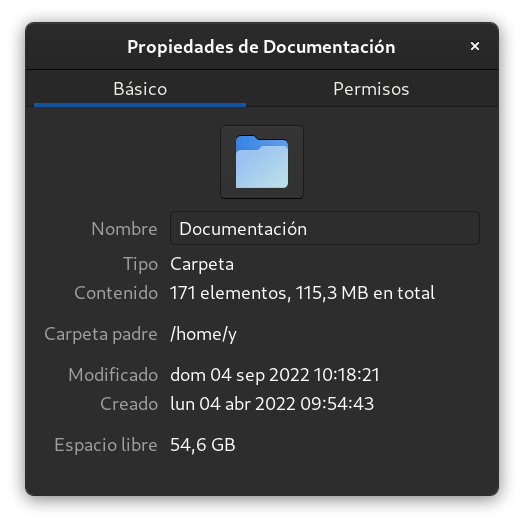
\includegraphics[width=0.4\linewidth]{hdd.png}
    \end{center}

    \item \textbf{Transmisión}: Cuando hablamos de tasa de transferencia de datos se hace uso del término “tasa de bits” (en inglés \textit{\textbf{bitrate}}), que indican el número de bits que se transmiten por unidad de tiempo. Hoy día se suele medir en kbps (o kb/s, kilobits por segundo), Mbps (Mb/s, o megabit por segundo), ... Para convertirlo a Bytes por segundo habría que dividirlo por “8”.

    \begin{center}
        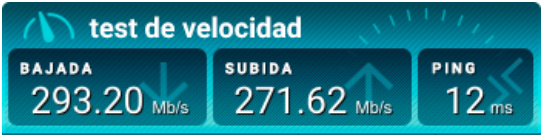
\includegraphics[width=0.4\linewidth]{bitrate.png}
    \end{center}

\end{itemize}

\warnbox{\textbf{La transmisión de datos se expresa en “bits por segundo”}}